\chapter{Introduction}

In this first chapter we want to familiarize the reader with the scientific
surrounding of our work. We hope to clarify what basic questions the physical
discipline of ultracold atom experiments tries to solve. In a second part we
want to elaborate on the concepts of localized optical potential dynamcis and
summarize the related work reported by the community.

\section{Background}

Many quantum systems studied in condensed matter physics are experimentally
challenging to access as any interactions can destroy the carefully prepared
quantum states. As a way forward, experiments with ultracold atoms in
optical lattices give us a highly controllable environment, permitting us to
simulate and explore quantum effects and expand our current understanding of
quantum mechanics and statistical physics \cite{Gross2017}.

\subsection{Ultracold atoms experiments}


\subsubsection{Apparatus}

The apparatus used for ultracold atoms experiments is a vacuum system that
cools down neutral atoms to temperatures of below micro Kelvin and loads them
into an optical lattice.

In \Cref{fig:ultracold_atoms_setup} a typical setup for an ultracold atoms
experiment is depicted. The oven on the left-hand side heats the atoms,
then a shutter selects atoms with correct momentum direction. The Zeeman
slower in the middle creates a magnetic field gradient such that the atoms
are always in resonance with the cooling laser antiparallel to the momentum
direction. In the \gls{mot} chamber atoms are cooled to target temperature
and loaded into the optical lattice \cite{Lewenstein2007}.

\begin{figure}[ht]
  \centering
  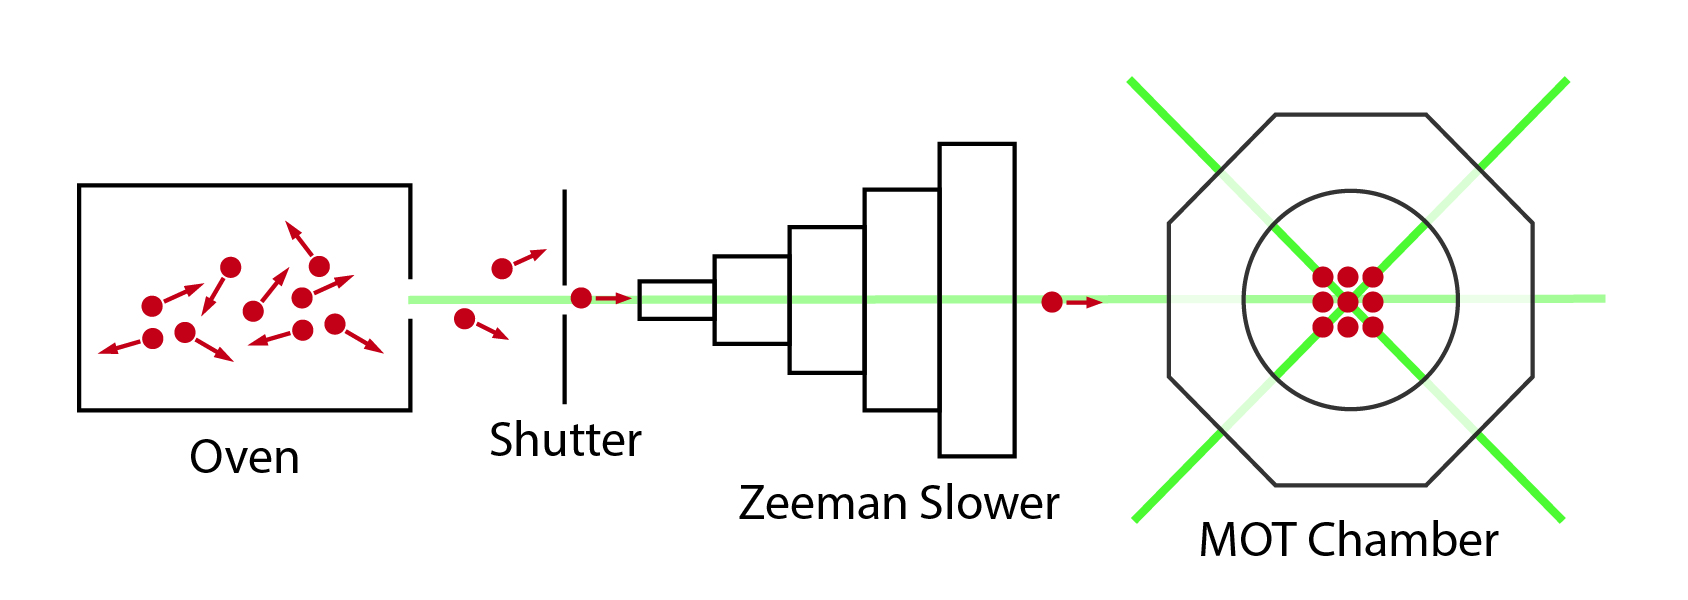
\includegraphics[width=\textwidth]{\mediadir{setup/ultracold-atoms.jpg}}
  \captionsetup{width=.8\textwidth}
  \caption{Typical setup of an ultracold atoms experiment. On the left-hand
  side an oven heats atoms that move towards a shutter. The shutter selects
atoms with momentum in direction of the \gls{mot}. A Zeeman slower creates
a magnetic gradient such that the atoms are in resonance with the cooling
laser antiparallel to their flight direction. Finally the atoms are loaded
into the optical lattice inside the \gls{mot} chamber.}
  \label{fig:ultracold_atoms_setup}
\end{figure}

In comparison to the dense energies occupied by atoms at usual room
temperature, low energy states are discrete such that quantum
behaviour dominates. In addition the low temperature of the atoms corresponds
to a low kinetic energy, thus suppressing the thermal motions of the atoms
such that they can be confined more easily to the optical lattice potential.

\subsection{Optical lattices}

\section{Concept}

\subsection{Related work}

Local manipulations of atoms inside optical lattices have been known for some
time in the embodiment of optical tweezers that allow trapping, stacking and
sorting of particles \cite{Tadmor2004}. Yet, only recently attempts to
interact with local particle clusters through high-precision time-averaged
optical potentials have been reported \cite{Roy2016}.

In the following we continue on the laid out work \cite{Hertlein2017} which
provided us with an optical setup for single-site manipulation using
\gls{aod} as well as considerations with regard to aperture limited
gaussian beam propagation.
